\documentclass[a4j, 11pt]{jarticle}
%#DVIPDF dvipdfmx -f ipa.map
\addtolength{\topmargin}{-2cm}
\addtolength{\textheight}{4cm}
\addtolength{\textwidth}{2cm}
\addtolength{\oddsidemargin}{-1cm}
%\addtolength{\evensidemargin}{-1cm}
%\title{}
%\author{}
\usepackage{ascmac}   % required for `\itembox'(yatex added)
\usepackage{lineno}
%\usepackage{minijs}   % font
\usepackage{multirow} 
\usepackage{graphicx} % required for `\includegraphics' (yatex added)
\usepackage{multicol} % required for `\multicols'(yatex added)
\usepackage{graphicx}
\pagestyle{empty}
\begin{document}
%\maketitle
\vspace*{1em}

\begin{table}[t]
 \scalebox{1.1}[1.2]{
  \begin{tabular}{|l|c|c|c|c|c|}
   \cline{1-5}
   ふりがな & \multicolumn{4}{|p{26em}|}{でんき つうしんだいがく}  & \multicolumn{1}{|c}{\multirow{5}{40mm}{ 
   \begin{minipage}{30mm}
    \centering
    \scalebox{0.4}{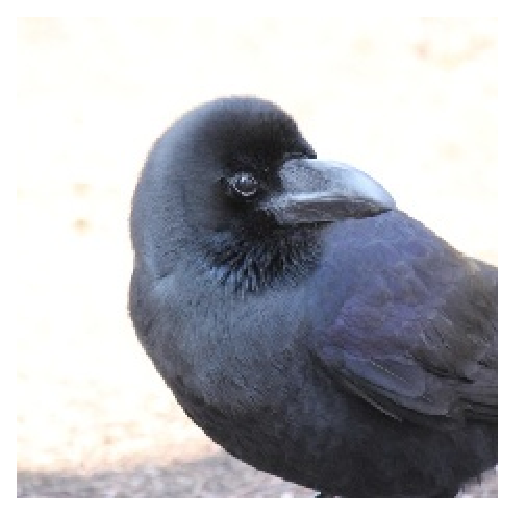
\includegraphics{./File/crow.eps}}
   \end{minipage}}} \\ \cline{1-5} 
   氏名 & \multicolumn{4}{|l|}{}\\ 

    & \multicolumn{4}{|l|}{\Large 電気 通信大学}\\ \cline{1-5}

   生年月日 &  \multicolumn{3}{|c|}{1918(大正7)年12月8日} & 男 \\ \cline{1-5}

   電話番号 & \multicolumn{4}{|l|}{042(443)5102}  \\ \cline{1-5}
   E-mail & \multicolumn{4}{|l|}{hogehogehoge@cs.euc.ac.jp}  \\ \hline

   ふりがな & \multicolumn{4}{|l|}{とうきょうと ちょうふし ちょうふがおか 1-5-1} & 電話 \\ \cline{1-5}

   郵便番号〒 & \multicolumn{4}{|l|}{182-8585} & \multirow{2}{*}{042(443)5102}\\ 
     & \multicolumn{4}{l|}{東京都調布市調布ヶ丘一丁目五番一号} & \\ \hline

   ふりがな & \multicolumn{4}{|l|}{} & 電話 \\ \cline{1-5}
   連落先〒 & \multicolumn{4}{|l|}{(現住所以外に連絡を希望する場合のみ記入)} & \multirow{2}{*}{042(443)5102} \\
   & \multicolumn{4}{|l|}{} & \\
   \hline
  \end{tabular}
}

\end{table}



\begin{table}[h]
 \begin{tabular}{|c|c|p{35em}|}
  \hline
  年& 月& \multicolumn{1}{|c|}{学歴,職歴}\\ \hline \hline
  & & \multicolumn{1}{|c|}{学歴} \\ \hline
  昭和24& 5&電気通信大学を設置, 電気通信学部を設置, 船舶通信専攻、陸上通信専攻、電波工学専攻を設置別科(通信専修)を設置 \\ \hline
  昭和26& 3&中央無線電信講習所を廃止 \\ \hline
  昭和26& 4&調布校舎を開校(東京都北多摩郡調布町) \\ \hline
  & & \\ \hline
  & & \\ \hline
  & & \\ \hline
  & & \\ \hline
  & & \\ \hline
  & & \\ \hline

 \end{tabular}
\end{table}
\begin{table}[h]
 \begin{tabular}{|c|c|p{35em}|}
  \hline
  年& 月& \multicolumn{1}{|c|}{免許,資格}\\ \hline \hline
  平成5& 4& ITパスポート 取得\\ \hline
  平成5& 7& 普通大型二輪免許 取得 \\ \hline
  平成7& 10& 基本情報技術 取得\\ \hline
  平成11& 4& TOEIC 400\\ \hline
  & & \\ \hline
  & & \\ \hline

 \end{tabular}
\end{table}

\begin{table}[p]
 \begin{tabular}{|ccc|}
\hline
  特技& & \\
  & & \\
  \multicolumn{3}{|p{40em}|}{\Large  私の特技は北斗百裂拳です。世紀末にはびこるスキンヘッドやモヒカン達を} \\ \hline
 \end{tabular}

\begin{tabular}{|ccc|}
\hline
 志望動機& & \\
 & & \\
  \multicolumn{3}{|p{40em}|}{\Large
 どっどど どどうど どどうど どどう
青いくるみも吹きとばせ
すっぱいかりんも吹きとばせ
どっどど どどうど どどうど どどう

 谷川の岸に小さな学校がありました。
 教室はたった一つでしたが生徒は三年生がないだけで、あとは一年から六年までみんなありました。運動場もテニスコートのくらいでしたが、すぐうしろは栗の木のあるきれいな草の山でしたし、運動場のすみにはごぼごぼつめたい水を噴く岩穴もあったのです。
 さわやかな九月一日の朝でした。青ぞらで風がどうと鳴り、日光は運動場いっぱいでした。黒い雪袴をはいた二人の一年生の子がどてをまわって運動場にはいって来て、まだほかにだれも来ていないのを見て、「ほう、おら一等だぞ。一等だぞ。」とかわるがわる叫びながら大よろこびで門をはいって来たのでしたが、ちょっと教室の中を見ますと、二人ともまるでびっくりして棒立ちになり、それから顔を見合わせてぶるぶるふるえましたが、ひとりはとうとう泣き出してしまいました。というわけは、そのしんとした朝の教室のなかにどこから来たのか、まるで顔も知らないおかしな赤い髪の子供がひとり、いちばん前の机にちゃんとすわっていたのです。そしてその机といったらまったくこの泣いた子の自分の机だったのです。} \\ \hline
\end{tabular}

\begin{tabular}{|ccc|}
\hline
本人希望記入欄 & & \\
 & & \\
  \multicolumn{3}{|p{40em}|}{\Large  } \\ \hline
\end{tabular}

\end{table}


\end{document} 
